% Copyright 2014 David W. Hogg (NYU).  All rights reserved.

\documentclass[pdftex]{beamer}
\usepackage{amssymb,amsmath,mathrsfs}
\usecolortheme{default}

% this one is debatable
\renewcommand{\emph}[1]{\textbf{#1}}

%%% color commands
\newcommand{\whiteonblack}{%
  \colorlet{fg}{white}
  \colorlet{bg}{black}
  \setbeamercolor{normal_text}{fg=white,bg=black}
  \setbeamercolor{background canvas}{fg=white,bg=black}
  \setbeamercolor{alerted_text}{fg=yellow}
  \setbeamercolor{example_text}{fg=white}
  \setbeamercolor{structure}{fg=white}
  \setbeamercolor{palette_quaternary}{fg=white}
}
\newcommand{\blackonwhite}{%
  \colorlet{fg}{black}
  \colorlet{bg}{white}
  \setbeamercolor{normal_text}{fg=black,bg=white}
  \setbeamercolor{background canvas}{fg=black,bg=white}
  \setbeamercolor{alerted_text}{fg=blue}
  \setbeamercolor{example_text}{fg=black}
  \setbeamercolor{structure}{fg=black}
  \setbeamercolor{palette_quaternary}{fg=black}
}
\xdefinecolor{pink}{rgb}{1.0,0.9,0.9}

%%% size and shape commands
\newlength{\figurewidth}
\setlength{\figurewidth}{0.9\textwidth}
\newlength{\figureheight}
\setlength{\figureheight}{0.9\textheight}

%%% text commands
\newcommand{\project}[1]{\textsl{#1}}
  \newcommand{\an}{\project{Astrometry.net}}
  \newcommand{\tc}{\project{The~Cannon}}
  \newcommand{\euclid}{\project{Euclid}}
  \newcommand{\flickr}{\project{flickr}}
  \newcommand{\gaia}{\project{Gaia}}
  \newcommand{\galex}{\project{GALEX}}
  \newcommand{\kepler}{\project{Kepler}}
  \newcommand{\GALEX}{\galex}
  \newcommand{\hst}{\project{HST}}
  \newcommand{\hipparcos}{\project{Hipparcos}}
  \newcommand{\lsst}{\project{LSST}}
  \newcommand{\sdss}{\project{SDSS}}
  \newcommand{\sdssiii}{\project{SDSS-III}}
  \newcommand{\sdssiv}{\project{SDSS-IV}}
  \newcommand{\boss}{\sdssiii\ \project{BOSS}}
  \newcommand{\osss}{\project{OSSS}}
  \newcommand{\ska}{\project{SKA}}
  \newcommand{\vo}{\project{VO}}
  \newcommand{\rttd}{\project{Right Thing To Do}$^{\mbox{\scriptsize\sffamily{TM}}}$}
\newcommand{\foreign}[1]{\textit{#1}}
\newcommand{\latin}[1]{\foreign{#1}}
  \newcommand{\cf}{\latin{cf.}}
  \newcommand{\eg}{\latin{e.g.}}
  \newcommand{\etal}{\latin{et~al.}}
  \newcommand{\etc}{\latin{etc.}}
  \newcommand{\ie}{\latin{i.e.}}
  \newcommand{\vs}{\latin{vs.}}

%%% math-mode commands
\newcommand{\unit}[1]{\mathrm{#1}}
  \newcommand{\rad}{\unit{rad}}
  \newcommand{\s}{\unit{s}}
  \newcommand{\yr}{\unit{yr}}
  \newcommand{\km}{\unit{km}}
  \newcommand{\kmps}{\km\,\s^{-1}}
\newcommand{\mmatrix}[1]{\boldsymbol{#1}}
\newcommand{\tv}[1]{\boldsymbol{#1}}
\newcommand{\dd}{\mathrm{d}}
\newcommand{\given}{\,|\,}
\newcommand{\Teff}{T_{\mathrm{eff}}}
\newcommand{\logg}{\log g}
\newcommand{\vsini}{v\,\sin i}
 % hogg standard colors
\setlength{\paperheight}{3.5in}
% 1.77778 is the ratio of 16 to 9
% 1.33333 is the ratio of 16 to 9
\setlength{\paperwidth}{1.33333\paperheight}
\setlength{\textwidth}{0.85\paperwidth}
\usepackage{amssymb,amsmath,mathrsfs}

\newcommand{\data}{\mbox{data}}
\newcommand{\pars}{\mbox{parameters}}

\title{Engineering considerations\\ for large astrophysics projects}
\author[David W. Hogg (NYU)]{David W. Hogg \\[1ex]
  \textsl{\small Center for Cosmology and Particle Physics\\
                 Department of Physics\\
                 New York University\\[1ex]
                 Max-Planck-Institut f\"ur Astronomie\\
                 Heidelberg, Germany}}
\date{2014 January 9}

\newcommand{\conclusionslide}{
\begin{frame}
  \frametitle{punchlines}
  \begin{itemize}
  \item Calibration programs are wasteful and \emph{reduce the accuracy} of your end-of-mission results.
    \begin{itemize}
    \item (you will need to adjust your observing strategy)
    \end{itemize}
  \item Homogeneity and uniformity of survey samples are \emph{impossible}, \emph{unnecessary}, and \emph{harmful} goals.
    \begin{itemize}
    \item (you will need to implement some probability theory)
    \end{itemize}
  \item Proper uncertainty propagation \emph{is not easy}.
    \begin{itemize}
    \item (I got nothing)
    \end{itemize}
  \item The challenge is to make precise measurements \emph{and} keep \emph{discovery space} open.
    \begin{itemize}
    \item (you will need to understand, quantitatively, your goals)
    \end{itemize}
  \end{itemize}
\end{frame}
}

\begin{document}

\begin{frame}
  \titlepage
\end{frame}

\conclusionslide

\begin{frame}
  \frametitle{my teachers (incomplete list)}
  \begin{itemize}
  \item Gerry Neugebauer (Caltech, emeritus)
  \item Sam Roweis (Toronto \& NYU, deceased)
  \item Dave~Schlegel~(LBL) \& Scott~Burles~(Cutler)
  \item Mike Blanton (NYU)
  \item Dustin~Lang~(CMU) \& Jo~Bovy~(IAS) \& Dan~Foreman-Mackey~(NYU)
  \end{itemize}
\end{frame}

\begin{frame}
  \frametitle{survey-centric context}
  \begin{itemize}
  \item \gaia
  \item \ska\ and pathfinders
  \item \euclid
  \item \lsst
  \item \sdssiv
    \begin{itemize}
    \item (I am going to get mean at the end.)
    \end{itemize}
  \end{itemize}
\end{frame}

\begin{frame}
  \frametitle{my day job}
  \begin{itemize}
  \item \an
  \item \project{emcee}
  \item precision measurement
  \item probabilistic inference
  \item data-driven models
  \item exoplanets and cosmology
  \end{itemize}
\end{frame}

\begin{frame}
  \frametitle{homogeneity and uniformity are impossible}
  \begin{itemize}
  \item weather
  \item target selection
  \item hardware evolution
  \item efficiency considerations
  \end{itemize}
\end{frame}

\begin{frame}
  \frametitle{probabilistic target selection}
  \begin{itemize}
  \item \sdssiii\ \boss\ quasar target selection
  \item in \sdss\ bandpasses, z~3 quasars look like A stars
  \item stars outnumber quasars enormously
  \item don't have good models of \emph{either}
    \begin{itemize}
    \item Bovy \etal\ arXiv:1011.6392
    \end{itemize}
  \item this target selection \emph{cannot be uniform}
    \begin{itemize}
    \item heterogeneous data quality means heterogeneous target selection
    \item star density varies on the sky
    \item suck it up!
    \end{itemize}
  \end{itemize}
\end{frame}

\begin{frame}
  \frametitle{homogeneity and uniformity are unnecessary}
  \begin{itemize}
  \item correct the data
    \begin{itemize}
    \item compute inverse selection ``volume'' or probabilities $1 / V_{\mathrm{max}}$ (ish)
    \item re-weight the data using these inverse volumes
    \item very \emph{wrong!}
    \end{itemize}
  \item forward modeling
    \begin{itemize}
    \item write down uncensored $p_0(\data\given\pars)$
    \item multiply by (one minus) censoring rate $\eta(\data)$
    \item renormalize to get expected $p(\data\given\pars)$
    \item this is a \emph{likelihood function}
    \end{itemize}
  \item (but: visualizing a forward model)
  \end{itemize}
\end{frame}

\begin{frame}
  \frametitle{estimators}
  \begin{itemize}
  \item Cram\`er--Rao bound
    \begin{itemize}
    \item example: \gaia\ astrometry
    \end{itemize}
  \item likelihood principle(s)
  \item it is \emph{our duty} to analyze our \emph{very limited data} with optimal methods
  \item the output of any data analysis must be a \emph{likelihood function}
    \begin{itemize}
    \item \project{WMAP}, \project{Planck}
    \end{itemize}
  \end{itemize}
\end{frame}

\begin{frame}
  \frametitle{likelihood principle}
  \begin{itemize}
  \item I said ``function''.
  \item $p(\data\given\pars)$
  \end{itemize}
\end{frame}

\begin{frame}
  \frametitle{living the likelihood dream}
  \begin{itemize}
  \item don't make a catalog of objects
    \begin{itemize}
    \item that's some kind of (probably inefficient) estimator
    \item even with error bars it can't transmit the full information
    \end{itemize}
  \item produce a likelihood function in \emph{catalog space}
    \begin{itemize}
    \item Lang \etal\ \url{http://TheTractor.org/}
    \item Brewer \etal\ arXiv:1211.5805
    \end{itemize}
  \end{itemize}
\end{frame}

\begin{frame}
  \includegraphics<1>[width=\textwidth]{brewer1.png}
  \includegraphics<2>[height=\textheight]{brewer2.png}
  \includegraphics<3>[width=\textwidth]{brewer3.png}
\end{frame}

\begin{frame}
  \frametitle{homogeneity and uniformity are unnecessary?}
  \begin{itemize}
  \item special case of two-point functions (and higher orders)
  \item currently an unsolved problem
    \begin{itemize}
    \item (but papers from Wandelt's group)
    \end{itemize}
  \end{itemize}
\end{frame}

\begin{frame}
  \frametitle{homogeneity and uniformity are harmful}
  \begin{itemize}
  \item can't be uniform in \emph{everything}
    \begin{itemize}
    \item the uniformity you choose only helps \emph{one} of your customers!
    \end{itemize}
  \item uniform samples end up requiring a lot of time on the least useful objects
  \item reduces the heterogeneity that is essential to calibration
  \end{itemize}
\end{frame}

\begin{frame}
  \frametitle{self-calibration}
  \begin{itemize}
  \item final imaging calibration of \sdss
    \begin{itemize}
    \item made \emph{no use at all} of the calibration program data
    \item Padmanabhan \etal\ arXiv:astro-ph/0703454
    \end{itemize}
  \end{itemize}
\end{frame}

\begin{frame}
picture from Padmanabhan
\end{frame}

\begin{frame}
  \frametitle{calibration programs are wasteful}
  \begin{itemize}
  \item there are \emph{more photons} in the science data
    \begin{itemize}
    \item therefore, the science data contain \emph{more information about calibration}
    \item (exceptions abound)
    \end{itemize}
  \item you must take your data with proper heterogeneity!
    \begin{itemize}
    \item \kepler
    \item tiling patterns
    \item Holmes \etal\ arXiv:1203.6255
    \end{itemize}
  \end{itemize}
\end{frame}

\begin{frame}
pictures from Holmes
\end{frame}

\begin{frame}
  \frametitle{target selection is classification}
  \begin{itemize}
  \item \sdssiii\ \boss\ is taking spectra of quasars, not stars
  \item stars outnumber (relevant) quasars by factors of hundreds
  \item observations are noisy and theoretical models are incomplete
  \item want to find \emph{only} the quasars\ldots or do we?
  \end{itemize}
\end{frame}

\begin{frame}
  \frametitle{classification algorithms}
  \begin{itemize}
  \item Support~Vector~Machine, Random~Forest, Artificial~Neural~Net
    \begin{itemize}
    \item all bad!
    \end{itemize}
  \item value of a \emph{causal} model
    \begin{itemize}
    \item training and test samples don't match
    \item need to classify new data taken under \emph{different conditions}
    \item make use of our technical knowledge about the data.
    \item Bovy \etal\ arXiv:1011.6392
    \end{itemize}
  \end{itemize}
\end{frame}

\begin{frame}
  ~ \hfill 1-epoch \hfill model \hfill 30-epoch
  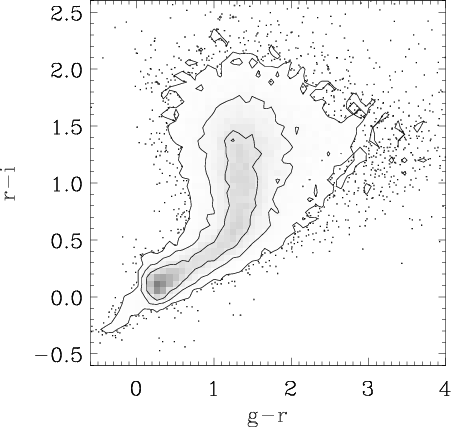
\includegraphics[width=0.35\textwidth,clip=]{single_data_200_i_202_ri_gr.png}%
  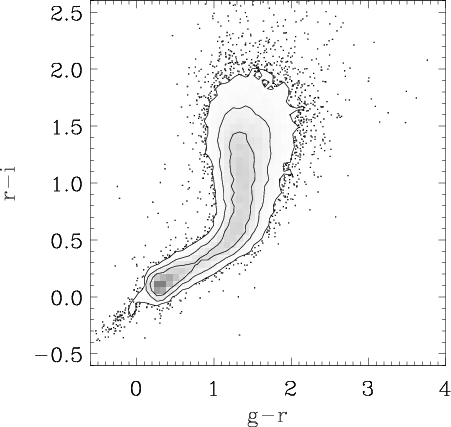
\includegraphics[width=0.35\textwidth,clip=]{coadd_data_200_i_202_ri_gr.png}%
  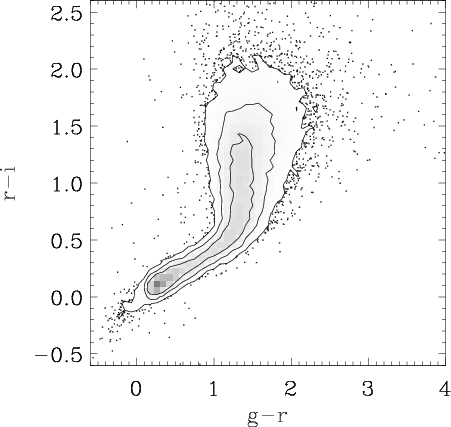
\includegraphics[width=0.35\textwidth,clip=]{dc_fluxdist_resample_200_i_202_20_ri_gr.png}
\end{frame}

\begin{frame}
  \includegraphics<1>[height=0.9\textheight]{xdstars.png}
  \includegraphics<2>[height=0.9\textheight]{xdqso.png}
  \includegraphics<3>[height=0.9\textheight]{xdqso_performance.png}
\end{frame}

\begin{frame}
  \frametitle{aside: discovery as classification}
  \begin{itemize}
  \item found an exoplanet?
    \begin{itemize}
    \item That's a model selection move.
    \item Bayes doesn't tell you how to \emph{make decisions}.
    \end{itemize}
  \item utility arises
    \begin{itemize}
    \item Make decisions that maximize expected (scientific?) return.
    \end{itemize}
  \item \an\ has an explicit utility model
    \begin{itemize}
    \item Automatic calibration of an image successful?
    \item Our ``customer model'' is that they are offended by false positives.
    \item Lang \etal\ arXiv:0910.2233
    \end{itemize}
  \end{itemize}
\end{frame}

\begin{frame}
  \frametitle{utility considerations}
  \begin{itemize}
  \item might be worth taking a source unlikely to be a quasar, as long as it is likely to be \emph{interesting}
    \begin{itemize}
    \item need to be able to make these trade-offs quantitatively
    \item requires a specification of \emph{utility}
    \item needs to be measured in dollars (or equivalent)
    \item long-term future discounted free cash flow
    \end{itemize}
  \item the ``game'' of proposal writing
    \begin{itemize}
    \item we aren't honest in our proposals about what we want
    \item \sdss\ was over-designed by any measure
    \item that was valuable!
    \end{itemize}
  \end{itemize}
\end{frame}

\begin{frame}
  \frametitle{over-design}
  \begin{itemize}
  \item \sdss\ was seriously over-designed to measure the large-scale structure
    \begin{itemize}
    \item (no-one thinks that was a bad idea)
    \item could have done all the large-scale structure in less than one year of observing
    \item we might have to be more honest going forward
    \end{itemize}
  \item if we want to use resources efficiently, we need to face a trade-off between efficiency and discovery
    \begin{itemize}
    \item At the present, everything is heuristics.
    \item I say we make this trade-off explicitly, not implicitly.
    \end{itemize}
  \end{itemize}
\end{frame}

\begin{frame}
  \frametitle{utopia}
  \begin{itemize}
  \item every part of your data analysis pipeline returns a likelihood function
    \begin{itemize}
    \item information propagation through the pipeline always by likelihood function
    \item implications are severe
    \end{itemize}
  \item you can simulate data under different experimental designs
    \begin{itemize}
    \item likelihood is $p(\data\given\pars)$
    \end{itemize}
  \item you have a specified utility function
    \begin{itemize}
    \item converts \emph{information} in your answer into \emph{dollars}
    \end{itemize}
  \item every decision can now be an optimization
    \begin{itemize}
    \item detectors, optical path, spectral elements
    \item filters, exposure times, cadences
    \item targets
    \end{itemize}
  \end{itemize}
\end{frame}

\begin{frame}
  \frametitle{example: bandpasses}
  \begin{itemize}
  \item \lsst\ plans to do imaging in $ugrizy$
  \item I am going to smash that $r$ filter!
  \item why not do $ugWizy$?
    \begin{itemize}
    \item easy example because zero-cost change
    \item doesn't require \emph{full} utility specification
    \item bet it is much better for low-$s/n$ objects
    \end{itemize}
  \end{itemize}
\end{frame}

\begin{frame}
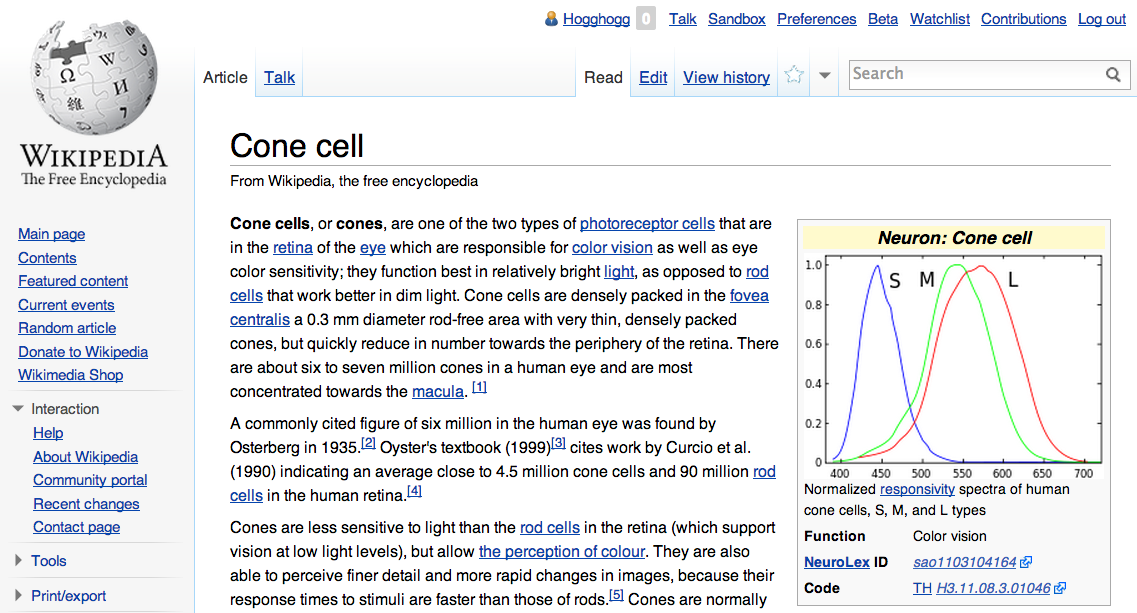
\includegraphics[width=\textwidth]{conecell.png}
\end{frame}

\begin{frame}
  \frametitle{hardware \foreign{vs} software trades}
  \begin{itemize}
  \item \project{P1640}
    \begin{itemize}
    \item Oppenheimer \etal\ arXiv:1303.2627
    \item Fergus \etal\ in prep
    \end{itemize}
  \item glitter cam
    \begin{itemize}
    \item Fergus \etal\ MIT-CSAIL-TR-2006-058
    \end{itemize}
  \end{itemize}
\end{frame}

\begin{frame}
  \includegraphics<1>[width=\figurewidth]{p1640data.png}
  \includegraphics<2>[width=\figurewidth]{p1640detections.png}
  \includegraphics<3>[width=\figurewidth]{p1640method.png}
  \includegraphics<4>[width=\figurewidth]{p1640spectra.png}
\end{frame}

\begin{frame}
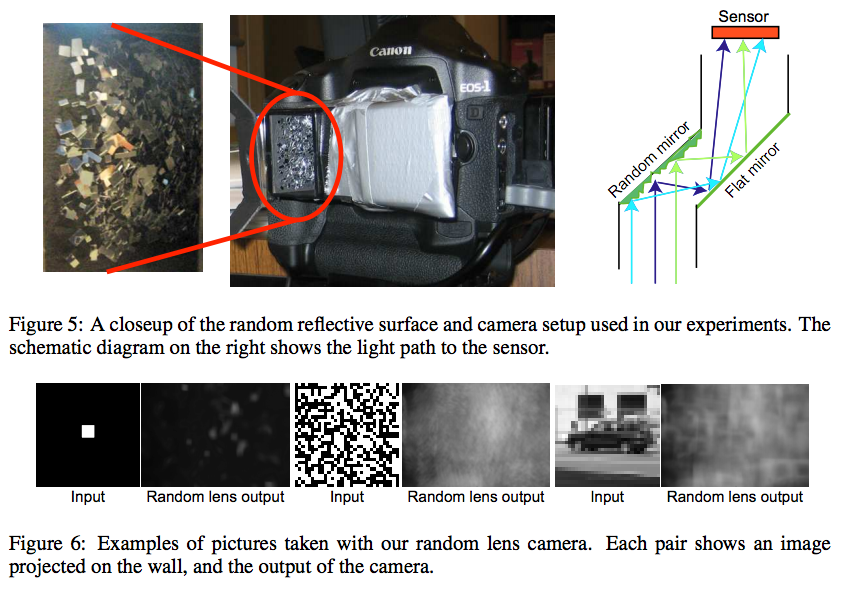
\includegraphics[width=\textwidth]{fergus.png}
\end{frame}

\begin{frame}
  \frametitle{open-source surveys}
  \begin{itemize}
  \item \hipparcos\ example
  \item \sdss\ calibration example
  \item enormous benefits accrue from making the data re-reducable from scratch
  \end{itemize}
\end{frame}

\begin{frame}
  \frametitle{throwing down the gauntlet}
  \begin{itemize}
  \item \gaia\ uncertainty propagation (qualitative)
  \item \euclid\ observing strategy for imaging
  \item \lsst\ bandpass, cadence, and exposure-time settings
  \item \ska\ pathfinder image products
  \item \project{eBOSS} two-point function estimators
  \item \project{APOGEE} \& \project{HERMES} signal-to-noise requirements
    \begin{itemize}
    \item (My hourly rates are a bargain.)
    \item (These surveys are all \emph{awesome}!)
    \end{itemize}
  \end{itemize}
\end{frame}

\conclusionslide

\end{document}
